\section{Detector and processing efficiencies}
\label{SEC:Efficiencies}

\subsection{Dataset and selection}

To determine the number of events expected both for signal and background processes, Monte Carlo samples of prompt $\phi$ and $D_s^\pm \rightarrow \phi \pi^\pm$ have been used. These Monte Carlo files contain $1\cdot10^4$ events each. 


\begin{center}
\resizebox{\textwidth}{!}{
\begin{tabular}{c|cc}
 & Prompt $\phi$ & $D_s^\pm \rightarrow \phi\pi^\pm$ \\ 
\hline 
$\pi$ from LL $K_S$ & TRGHOSTPROB $<$ 0.35 & TRGHOSTPROB $<$ 0.35\\
& P $>$ 2\,GeV & P $>$ 2\,GeV \\
& MIPCHI2DV(PRIMARY) $>$ 9& MIPCHI2DV(PRIMARY) $>$ 9\\
\hline 
$\pi$ from DD $K_S$ & P $>$ 2\,GeV & P $>$ 2\,GeV \\
& MIPCHI2DV(PRIMARY) $>$ 4& MIPCHI2DV(PRIMARY) $>$ 4\\
\hline 
$K_S$ &ADOCACHI2CUT(25, '')&ADOCACHI2CUT(25, '')\\
&VFASPF(VCHI2) $<$ 25&VFASPF(VCHI2) $<$ 25\\
&PT $>$ 500\,MeV&PT $>$ 500\,MeV\\
&ADMASS('KS0') $<$ 20\,MeV&ADMASS('KS0') $<$ 20\,MeV\\
&BPVVD $>$ 10\,mm&BPVVD $>$ 10\,mm\\
&BPVVDCHI2 $>$ 50&BPVVDCHI2 $>$ 50\\
&VFASPF(VCHI2PDOF) $<$ 10 &VFASPF(VCHI2PDOF) $<$ 10\\
&BPVDIRA $>$ 0.9999&BPVDIRA $>$ 0.9999\\
\hline
$\phi$ & LL LL or LL DD combinations & LL LL or LL DD combinations\\
&APT $>$ 1000\,MeV & APT $>$ 1000\,MeV\\
&AM $<$ 1100\,MeV & AM $<$ 1100\,MeV\\
&ACUTDOCACHI2(100,'') & ACUTDOCACHI2(100,'')\\ 
&M $<$ 1070\,MeV & M $<$ 1090\,MeV\\
&VFASPF(VCHI2/VDOF) $<$ 10 & VFASPF(VCHI2/VDOF) $<$ 10\\
&MIPCHI2DV(PRIMARY) $<$ 100 & MIPCHI2DV(PRIMARY) $<$ 100\\
\hline
$\pi$ from $D_s$ &&PT $>$ 250\,MeV\\
&&MIPCHI2DV(PRIMARY) $>$ 4\\
&&MIPCHI2DV(PRIMARY) $<$ 300\\
&&TRGHOSTPROB $<$ 0.35\\
\hline
$D_s$ &&APT $>$ 800\,MeV\\
&&ADAMASS(1920\,MeV) $<$ 130\,MeV\\
&&ACUTDOCACHI2(100,'')\\
&&DMASS(1920\,MeV) $<$ 100\,MeV\\
&&VFASPF(VCHI2/VDOF) $<$ 10\\
&&MIPCHI2DV(PRIMARY) $<$ 100\\
\hline
Post-stripping cuts & $\SI{1010}{MeV}<$phi\_M$<\SI{1030}{MeV}$ &$\SI{1010}{MeV}<$phi\_M$<\SI{1030}{MeV}$\\
&&\SI{1955}{MeV}$<$Ds\_M$<$\SI{1985}{MeV}\\
&&IPCHI2 $\geq$ 15
\end{tabular} }
\captionof{table}{Summary of all cuts done in the stripping line and in post-stripping selection, both for prompt $\phi$ and $D_s^\pm\rightarrow\phi\pi^\pm$.}\label{TAB:Stripping}
\end{center}

For the selection the stripping line \verb!PhiToKSKS! has been used. The version used in this study is not the final one. It can be found at \url{https://github.com/gdujany/phi2KsKs/blob/master/StrippingPhiToKSKS.py}. A summary of the cuts in the stripping line are given in table \ref{TAB:Stripping}.





\begin{center}
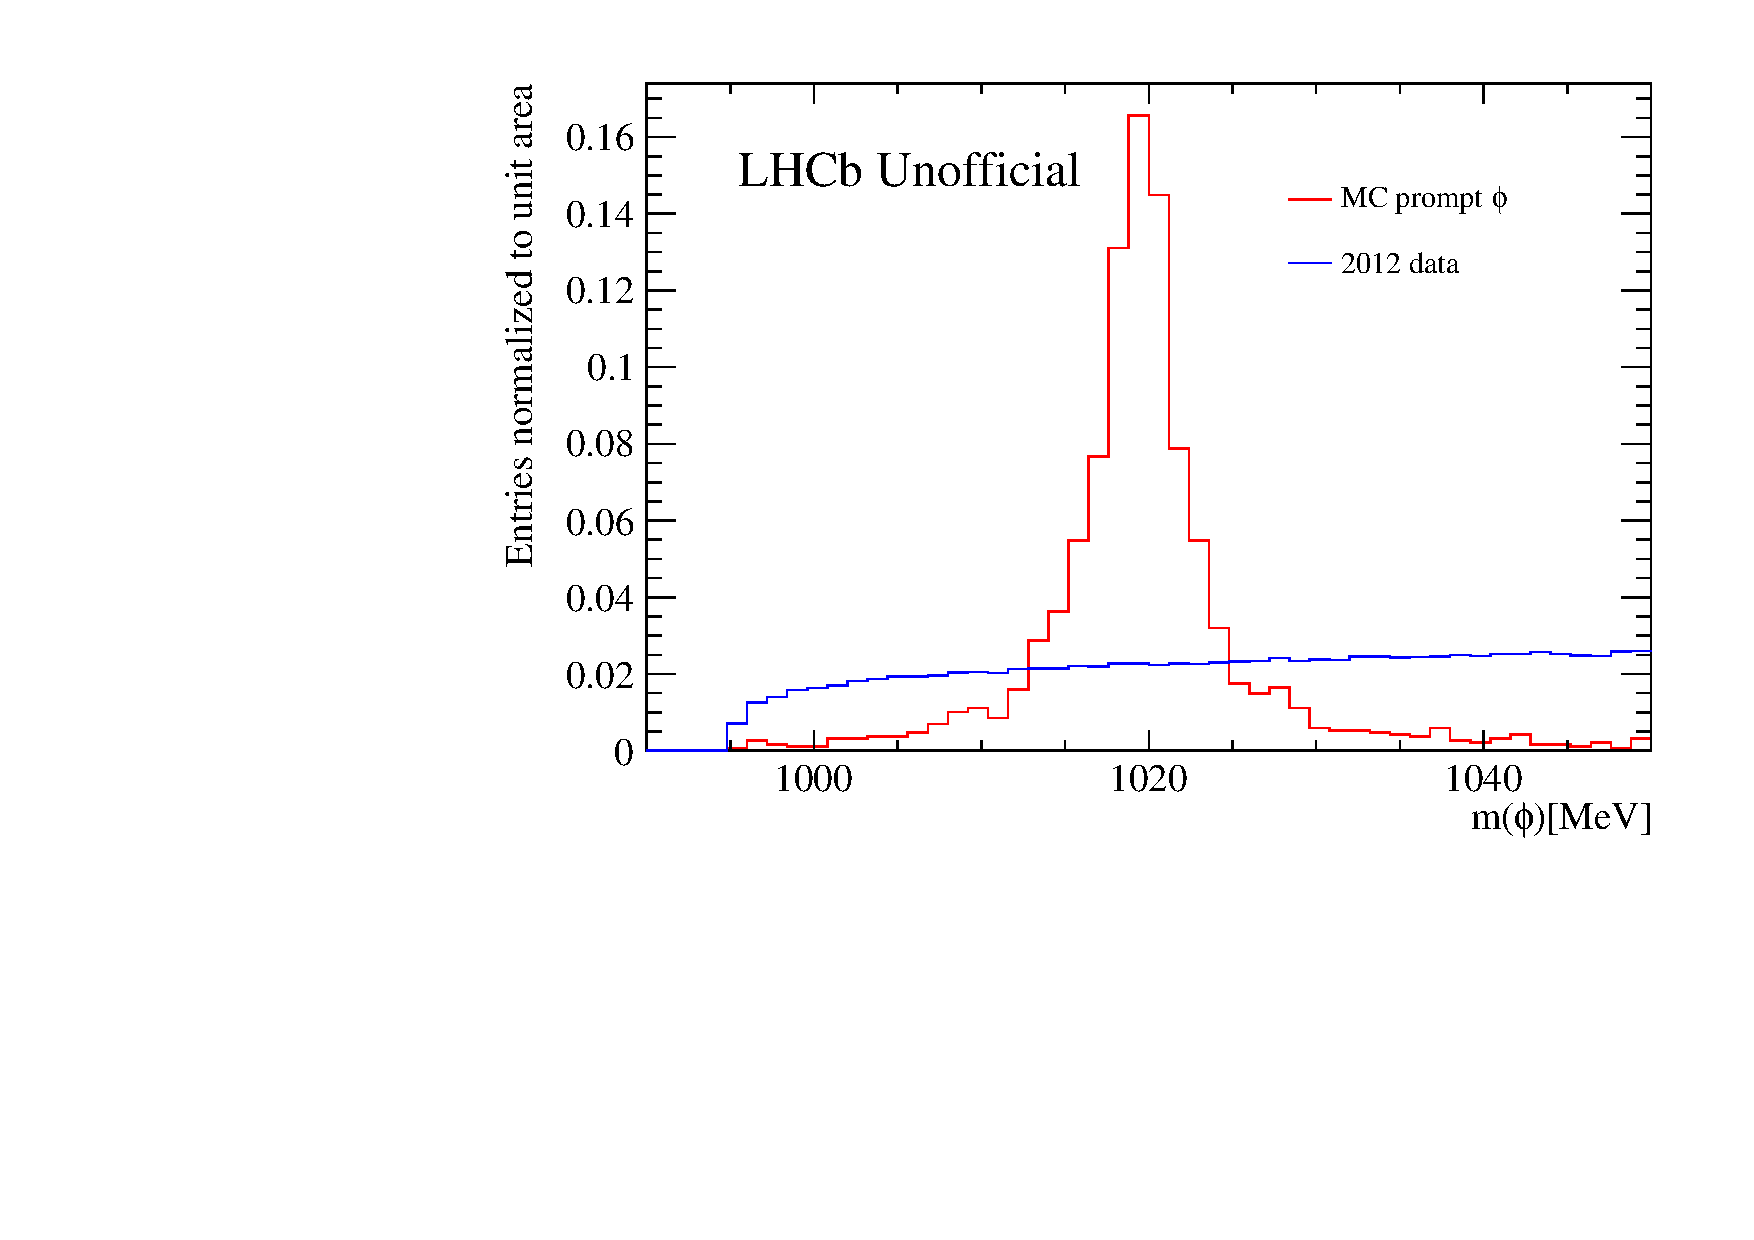
\includegraphics[height = .49\textwidth]{figs/m_phi_incl.pdf}
\captionof{figure}{Invariant mass of $\phi$ after applying the selection. The Monte Carlo shows the spectrum for $\phi\rightarrow K_SK_S\rightarrow \pi^+\pi^-\pi^+\pi^-$ whereas the 2012 data contains mostly background events.}\label{FIG:IM1}
\end{center}

\begin{center}
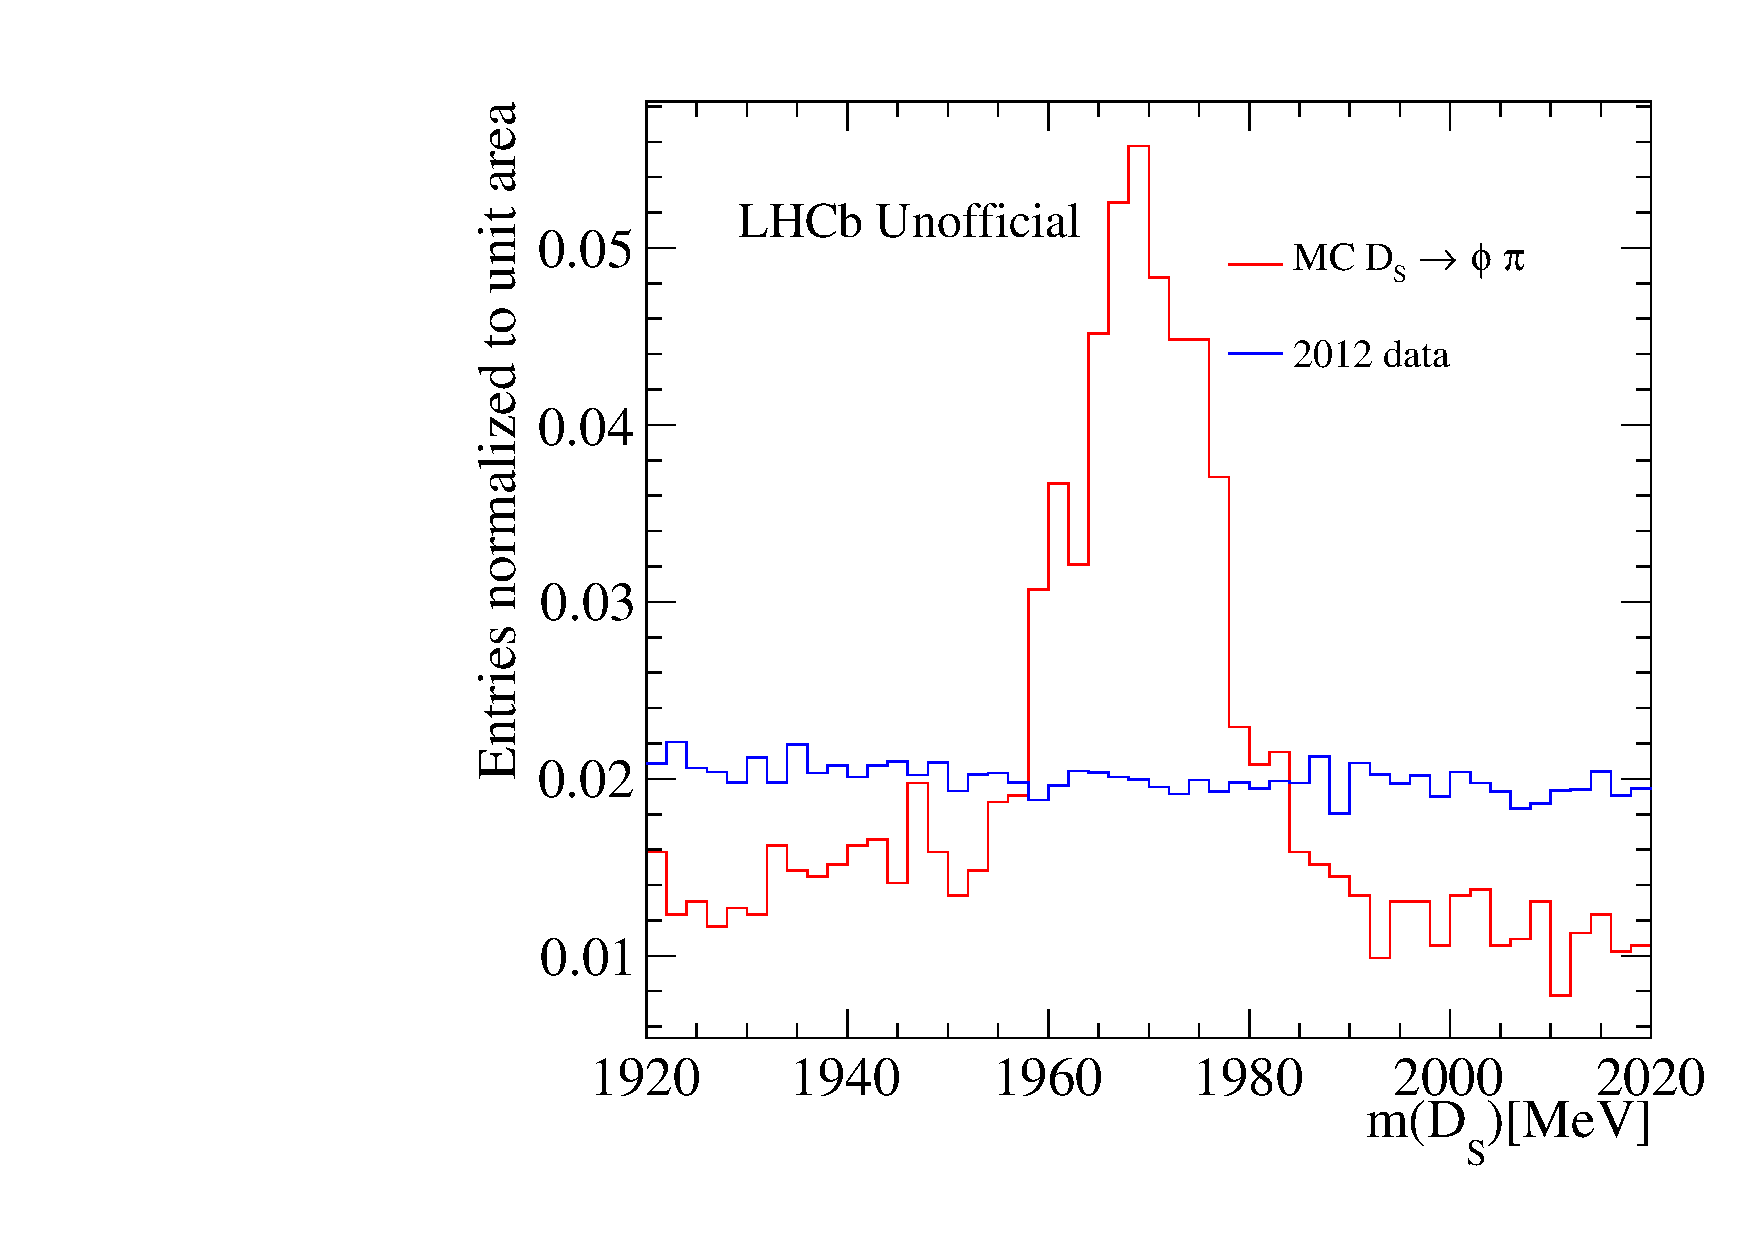
\includegraphics[width = .49\textwidth]{figs/m_Ds_Ds.pdf}
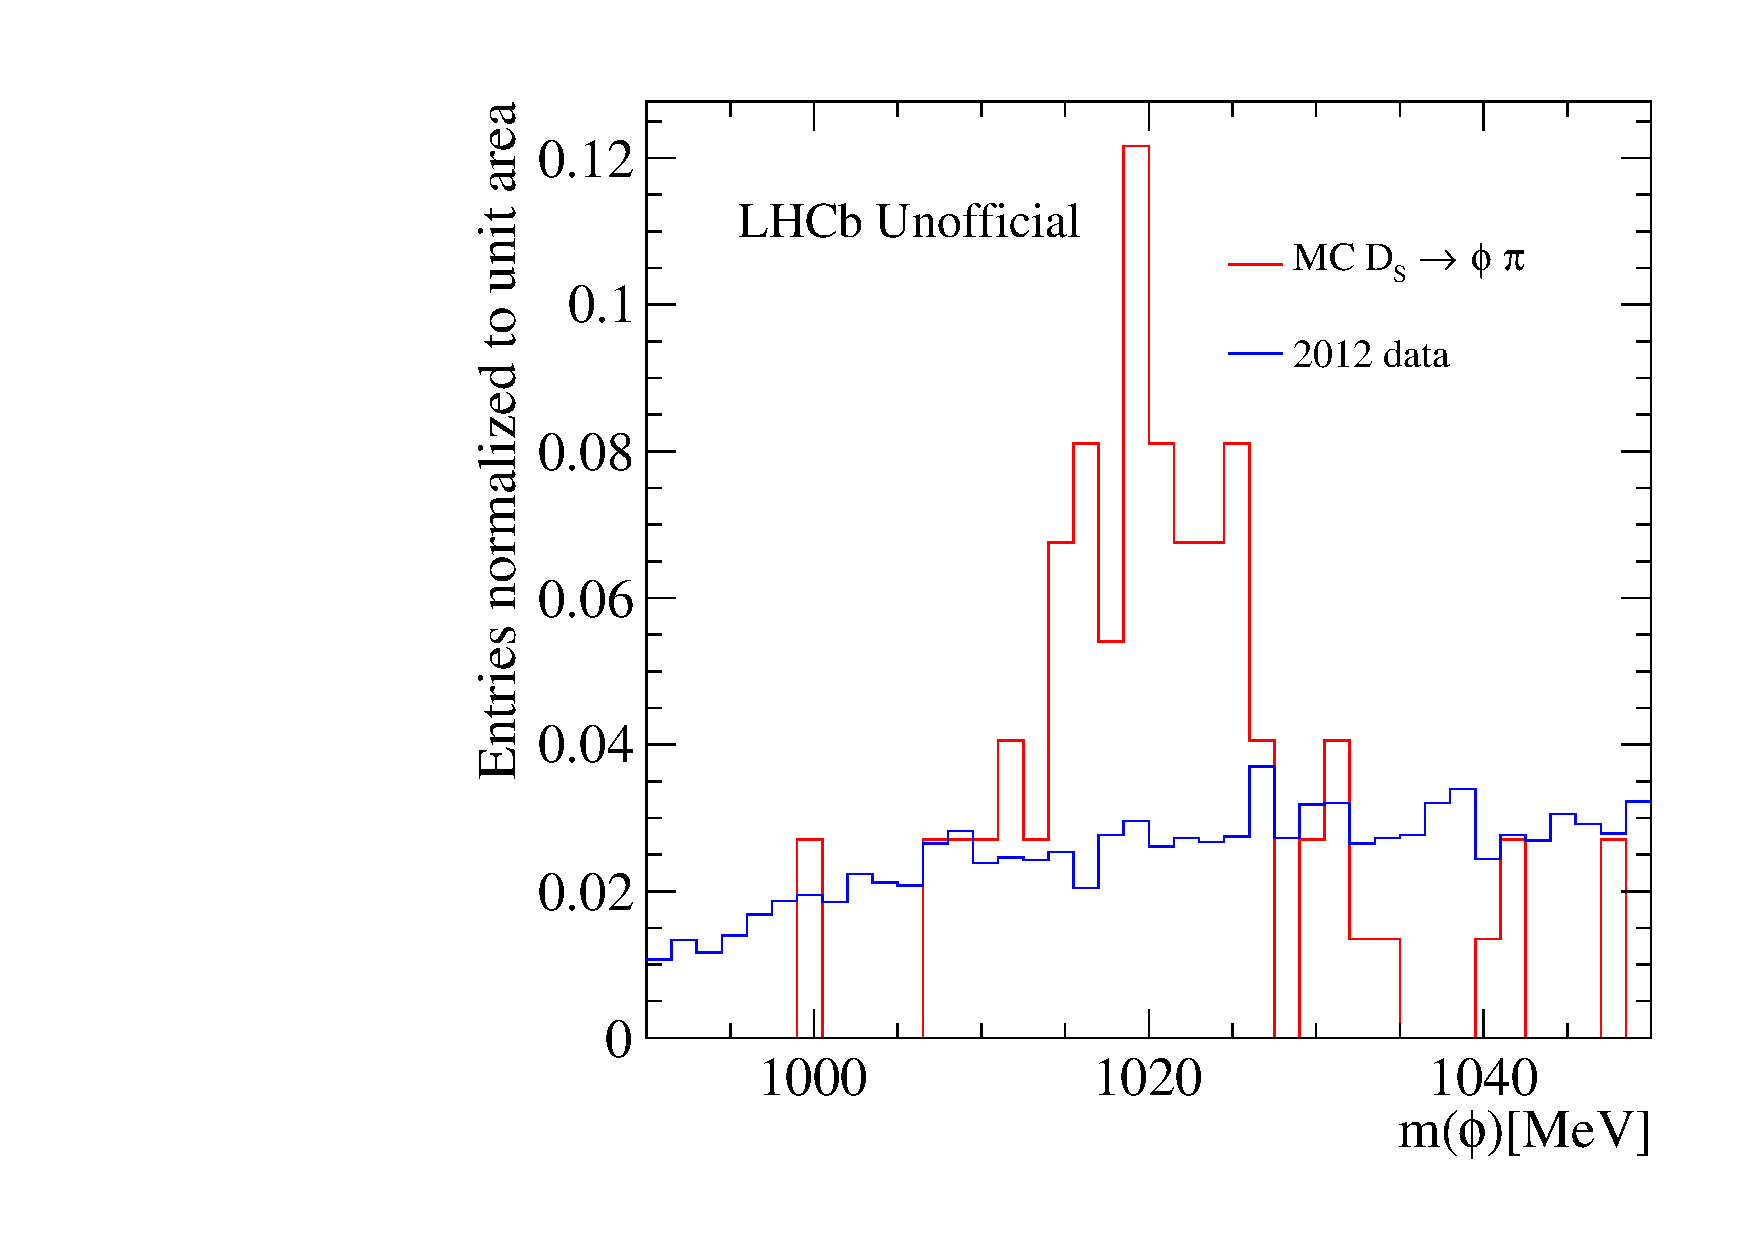
\includegraphics[width = .49\textwidth]{figs/m_phi_Ds.pdf}
\captionof{figure}{Invariant mass of $D_s$ and $\phi$ after applying the selection. The Monte Carlo shows the spectra for $D_s^\pm \rightarrow \phi\pi^\pm\rightarrow K_SK_S\rightarrow \pi^+\pi^-\pi^+\pi^-\pi^\pm$ whereas the 2012 data contains mostly background events.}\label{FIG:IM2}
\end{center}

The mass windows used for all following studies are $\SI{1010}{MeV} < m(\phi) < \SI{1030}{MeV}$ and $\SI{1955}{MeV} < m(D_s^\pm) < \SI{1985}{MeV}$. In order to reject prompt $\phi$, in the $D_s^\pm \rightarrow \phi \pi^\pm$ selection the cut $\chi^2 \geq 15$ on the $\chi^2$ of a fit matching the $\phi$ origin vertex to the primary vertex was added. 


The 2012 data set was processed with the selection as well. For the prompt $\phi$ selection, the \verb!CHARM.mDST! container was used, as was the \verb!CHARMCOMPLETEEVENT.DST! container for the $D_s^\pm \rightarrow \phi \pi^\pm$ selection (both are \verb!Reco14!). The resulting spectra of the invariant masses of $\phi$ and $D_s^\pm$ normalized to unit area can be found in figures \ref{FIG:IM1} and \ref{FIG:IM2}.


\subsection{Efficiencies}
The reconstruction and trigger efficiencies have been determined from the Monte Carlo samples. The probabilities of the kaon decays have been determined using the decay intensities in equation \eqref{EQ:DI1} and \eqref{EQ:DI2}, with 
$\zeta_{SL}$ set to 0.098, the 95\% C.L. limit set by KLOE. It is estimated that to decay, on 
average, inside the beampipe, the decay time of the kaons has to be less than 25\,ps, and to be reconstructed at all, the decay time has to be less than 200\,ps. The estimate for the background yield is the number of events in the 2012 data after applying the selection. All resulting values can be found in table \ref{TAB:Efficiencies}.


\begin{center}
\resizebox{\textwidth}{!}{
\begin{tabular}{ccc}
&Prompt $\phi$ & $D_s \rightarrow \phi \pi$ \\
\hline 
\hline
\vspace*{-6pt}\\
Cross section (\SI{14}{TeV}), LHCb acceptance &\SI{ 3516 }{\micro\barn} & \SI{ 388 }{\micro\barn} \\
\hline
Branching fractions & 34.2\% & 4.5\% $\cdot$  34.2\% \\
\hline
Fiducial cuts efficiency & 2.5\% & 7.0\%\\
\hline
Probability $K_sK_s \rightarrow 4\pi$, \\
 exactly 1 (2) decays inside beampipe &\multicolumn{2}{c}{$ 15.1\%$ ( $2.8\%$ )} \\
\hline
Probability $K_sK_L \rightarrow 4\pi$ (CPV),\\
exactly 1 (2) decays inside beampipe &\multicolumn{2}{c}{$ 3.98\cdot 10^{-7}$ ( $4.99\cdot 10^{-10}$ )} \\
\hline
Upper limit KLOE probability\\ $K_sK_L \rightarrow 4\pi$ (CPV 
+ CPTV),\\ exactly 1 (2) decays inside beampipe &\multicolumn{2}{c}{$  5.13\cdot 10^{-7}$ ( $1.64\cdot 10^{-8}$ )}\\
\hline
Reconstruction \& selection efficiency &  7.9\% ( 7.6\% )  & 1.4\% ( 3.9\% )\\
L0 efficiency&  16.1\% ( 18.6\% )&  23.0\% ( 19.5\% )\\
HLT1 efficiency&  13.7\% ( 16.7\% )& 35.6\% ( 25.0\% )\\
HLT2 efficiency&  65.6\% ( 100.0\% )& 68.8\% ( 100.0\% )\\
\hline
Total efficiency &$ 4.39\cdot 10^{-5} $ ( $ 5.85\cdot 10^{-5} $ )&$ 8.18\cdot 10^{-5} $ ( $ 1.32\cdot 10^{-4} $ )\\
Expected events SM background / fb$^{-1}$ &$ 21 $ ( $ 3.51\cdot 10^{-2} $)&$ 1.94\cdot 10^{-1} $ ( $ 3.94\cdot 10^{-4} $)\\
Upper limit for SM background + signal (KLOE)  / fb$^{-1}$ &$ 27 $ ( $ 1.15 $ )&$ 2.5\cdot 10^{-1} $ ( $ 1.29\cdot 10^{-2} $ )\\
Combinatoric background (data 2012) / fb$^{-1}$ & 163110 ( 29120 ) &  450 ( 2030 )\\
\end{tabular}
}
\captionof{table}{Cross sections, branching fractions, efficiencies and resulting event yields for signal, standard model background, and combinatoric background. If two numbers are given, the one in brackets assumes two kaons decaying inside the beampipe, whereas for the other it is required that exactly one of the two kaons decays inside the beampipe.}\label{TAB:Efficiencies}
\end{center}
\newpage
From the event yield one can conclude that the signal to background ratio is in the same order of magnitude for both approaches and not much is gained from using the $D_s^\pm \rightarrow \phi \pi^\pm$ approach.